\chapter{System analysis and design}
\section{System analysis}
As indicated earlier, the system was developed in three major iterations. However, before the
iterations had begun, initial requirement gathering and analysis was done. This covered the whole
system.
Initial requirement gathering and analysis
Functional requirements:
Nonfunctional requirements:
Constraints (“Pseudo requirements”):
Iteration 1
This iteration involved the development of the web crawler module of the system.
Requirements
Functional requirements
crawl webpages in any domain given a base url
take into account rich files i.e. pdf, doc,xls,
discard similar pages
resilient to network outages (saves state)
Non-functional requirements
minimal traffic
not overload servers
able to start/pause/resume/stop/resume on demand
avoid getting banned
Iteration 2
This iteration involved the development of the data analysis module.
Iteration 3
This iteration involved the development of the data presentation module
usecases
\begin{figure}
	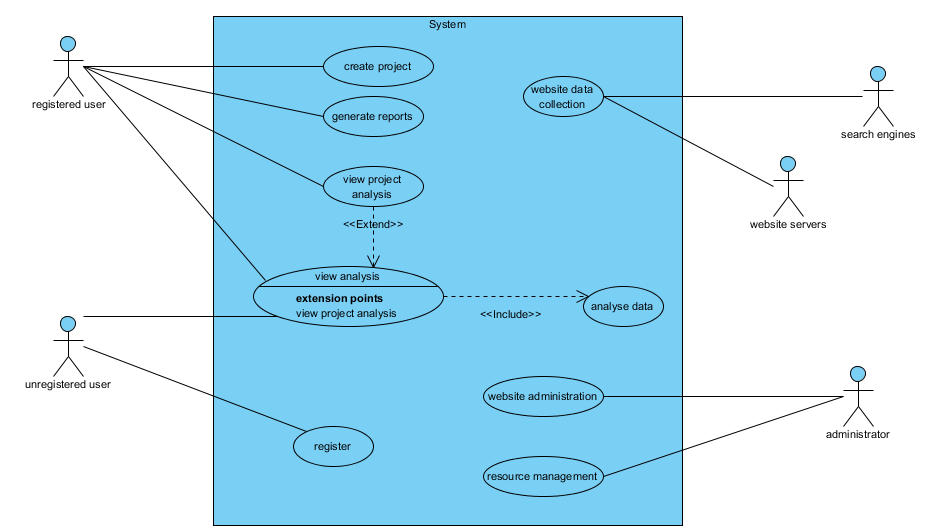
\includegraphics[width=\linewidth]{usecase.png}
	\caption{System use case model}
\end{figure}

\begin{tabular}{ l | c || r }
  1 & 2 & 3 \\
  4 & 5 & 6 \\
  7 & 8 & 9 \\
\end{tabular}

\section{System design}

